

%\documentclass[a4paper]{jarticle}

\section{mpie.rb Draw pie graph\label{sect:mpie}}
\index{mpie@mpie}

The command draws a pie chart. 
By specifying the attributes assigned to x axis and y axis,  users can create 1 dimensional or 2 dimensional pie matrix. 
The output of the graph is saved as HTML file which can be displayed in popular browsers. 

The input data in CSV format is shown in Table \ref{tbl:mpie_input2}. The fields that construct the pie chart can be specified at \verb|f=| parameter. 
The attributes assigned to x-axis and y-axis can be specified in \verb|k=| parameter. 
When one field is specified at \verb|k=| parameter, one-dimensional pie chart matrix is created, 
if two fields are specified at \verb|k=| parameter, two-dimensional pie chart matrix is created. 
When \verb|k=| parameter is not specified, one pie chart is created. 

The pie chart is created with the JavaScript library D3.js (Data-Driven Documents). Please refer to the official website of D3.js  (\url{http://d3js.org/}) for more details.   
 Note that Nysol/mcmd library is required for this command. 
 

\begin{table}[http]
\begin{center}
\caption{Number of individuals by age  and prefecture \label{tbl:mpie_input2}}
{\small
\begin{tabular}[t]{ccr}
\hline
Pref&Age&Population \\
\hline
Nara&10&310504\\
Nara&20&552339\\
Nara&30&259034\\
Nara&40&450818\\
Nara&50&1231572\\
Nara&60&1215966\\
Nara&70&641667\\
Hokkaido&10&310504\\
Hokkaido&20&252339\\
Hokkaido&30&859034\\
Hokkaido&40&150818\\
Hokkaido&50&9231572\\
Hokkaido&60&4215966\\
Hokkaido&70&341667\\
\hline
\end{tabular}
}
\end{center}
\end{table}

\newpage
\subsection{Format}
\begin{verbatim}
  mpie.rb [i=] f= v= [o=] [k=] [title=] [pr=] [cc=] [--help]
\end{verbatim}

\begin{table}[htbp]
{\small
\begin{tabular}{ll}
\verb|i=|        & Input data file name  (CSV format) \\
\verb|f=|        & Specify the field name of component. \\
                 & Null data is ignored. \\
\verb|v=|        & Specify the field name of component ratio (item that determines the arc length of the pie chart).\\
                 & Data is treated as zero if it consists of null value.  \\
                 & Values started with 0 is ignored. Values except numeric characters returns error. \\
\verb|o=|        & Output file name (HTML file) \\
\verb|k=|        & Specify two or less field names assigned to x-axis and y-axis. \\
                 & Create one pie chart when this parameter is not specified. \\
                 & Create a one-dimensional pie chart when one field is specified, \\
                 & create two-dimensional pie chart when two fields are specified. \\
\verb|title=|    & Specify the title of the graph\\
\verb|pr=|       & Specify the radius of the pie chart (default is 160).  \\
\verb|cc=|       & Specify the maximum number of pie charts to be displayed in 1 row (default is 5). \\
                 & Specify for one-dimension pie chart matrix. \\
\verb|--help|    &  Show help \\
\end{tabular} 
}
\end{table} 

Noted that in \verb|mpie.rb| command, 
the fields specified in \verb|f=| parameter  and \verb|k=| parameter do not have automatic sorting function. 
It is necessary to sort the data prior to this command as needed. 

\subsection{Examples}
\subsubsection*{例1: 円グラフを1つ描画する}

\verb|dat1.csv|ファイルの\verb|Age|を構成要素項目に、
\verb|Population|を構成比項目として円グラフを1つ描画する。

\begin{Verbatim}[baselinestretch=0.6,frame=single]
$ more dat1.csv
Age,Population
10,310504
20,552339
30,259034.5555
40,0450818
50,1231572
60,1215966
70,641667
$ mpie.rb i=dat1.csv v=Population f=Age o=result1.html
#END# mpie.rb i=dat1.csv v=Population f=Age o=result1.html;
\end{Verbatim}

以下の円グラフが描画される。

ブラウザで表示した円グラフにマウスカーソルを置くと、
構成要素項目とその構成比がポップアップで表示される。
グラフはマウスによるドラッグ操作で移動することができ、
またマウスのスクロール操作によって拡大縮小もできる。

\begin{flushleft}
\fbox{
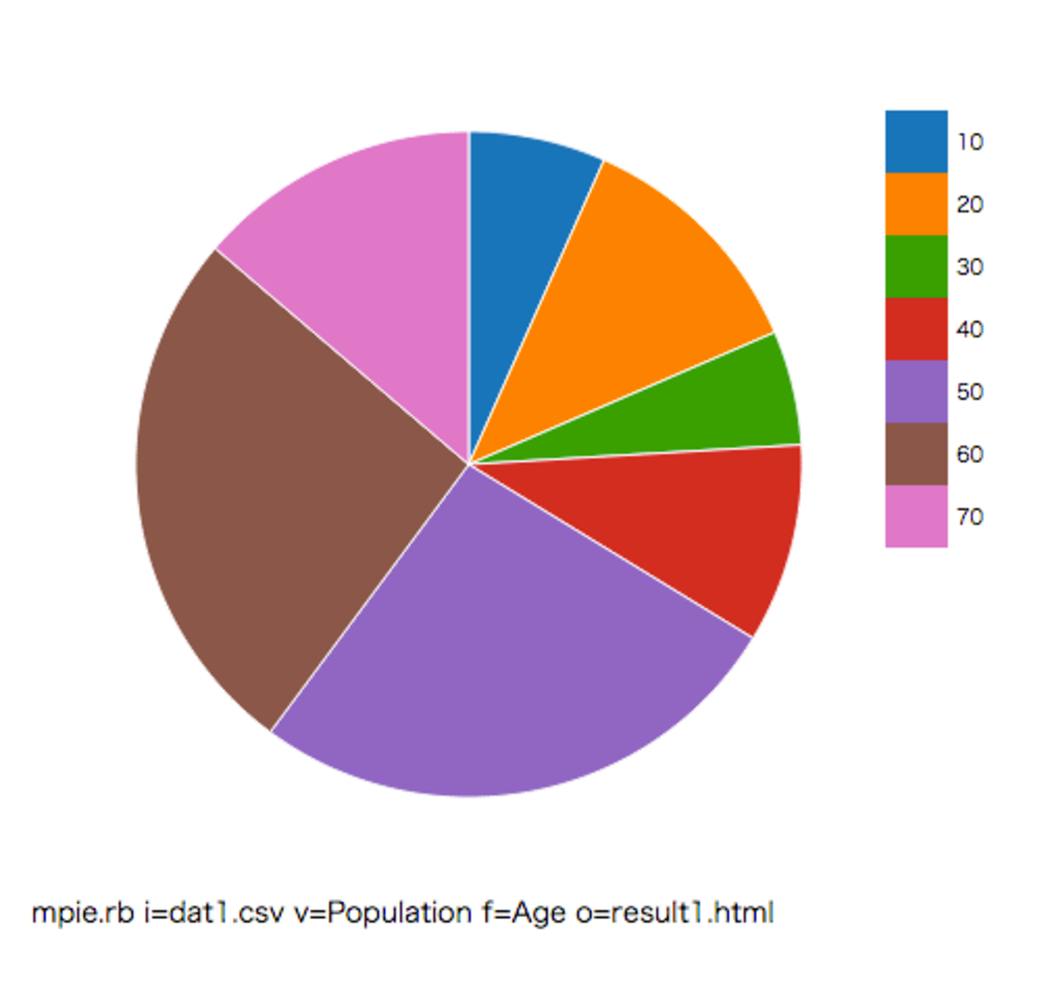
\includegraphics[scale=0.7]{figure/mpie1.eps}
}
\end{flushleft}

\subsubsection*{例2: 1次元の円グラフ行列を描画する}

\verb|dat2.csv|ファイルの\verb|Age|を構成要素項目に、
\verb|Population|を構成比項目として円グラフを描画する。
\verb|k=|パラメータに\verb|Pref|項目を指定しているので、
\verb|Pref|項目の値をx軸(横方向)に展開した1次元の円グラフ行列が描画される。
\verb|title=|パラメータでグラフのタイトルも指定している。

\begin{Verbatim}[baselinestretch=0.5,frame=single]
$ more dat2.csv
Pref,Age,Population
奈良,10,310504
奈良,20,552339
奈良,30,259034
奈良,40,450818
奈良,50,1231572
奈良,60,1215966
奈良,70,641667
北海道,10,310504
北海道,20,252339
北海道,30,859034
北海道,40,150818
北海道,50,9231572
北海道,60,4215966
北海道,70,341667
$ mpie.rb i=dat2.csv k=Pref v=Population f=Age o=result2.html
 title=奈良と北海道の年代ごとの人口
#END# mpie.rb i=dat2.csv k=Pref v=Population f=Age o=result2.html 
title=奈良と北海道の年代ごとの人口;
\end{Verbatim}

以下の円グラフ行列が描画される。

\begin{flushleft}
\fbox{
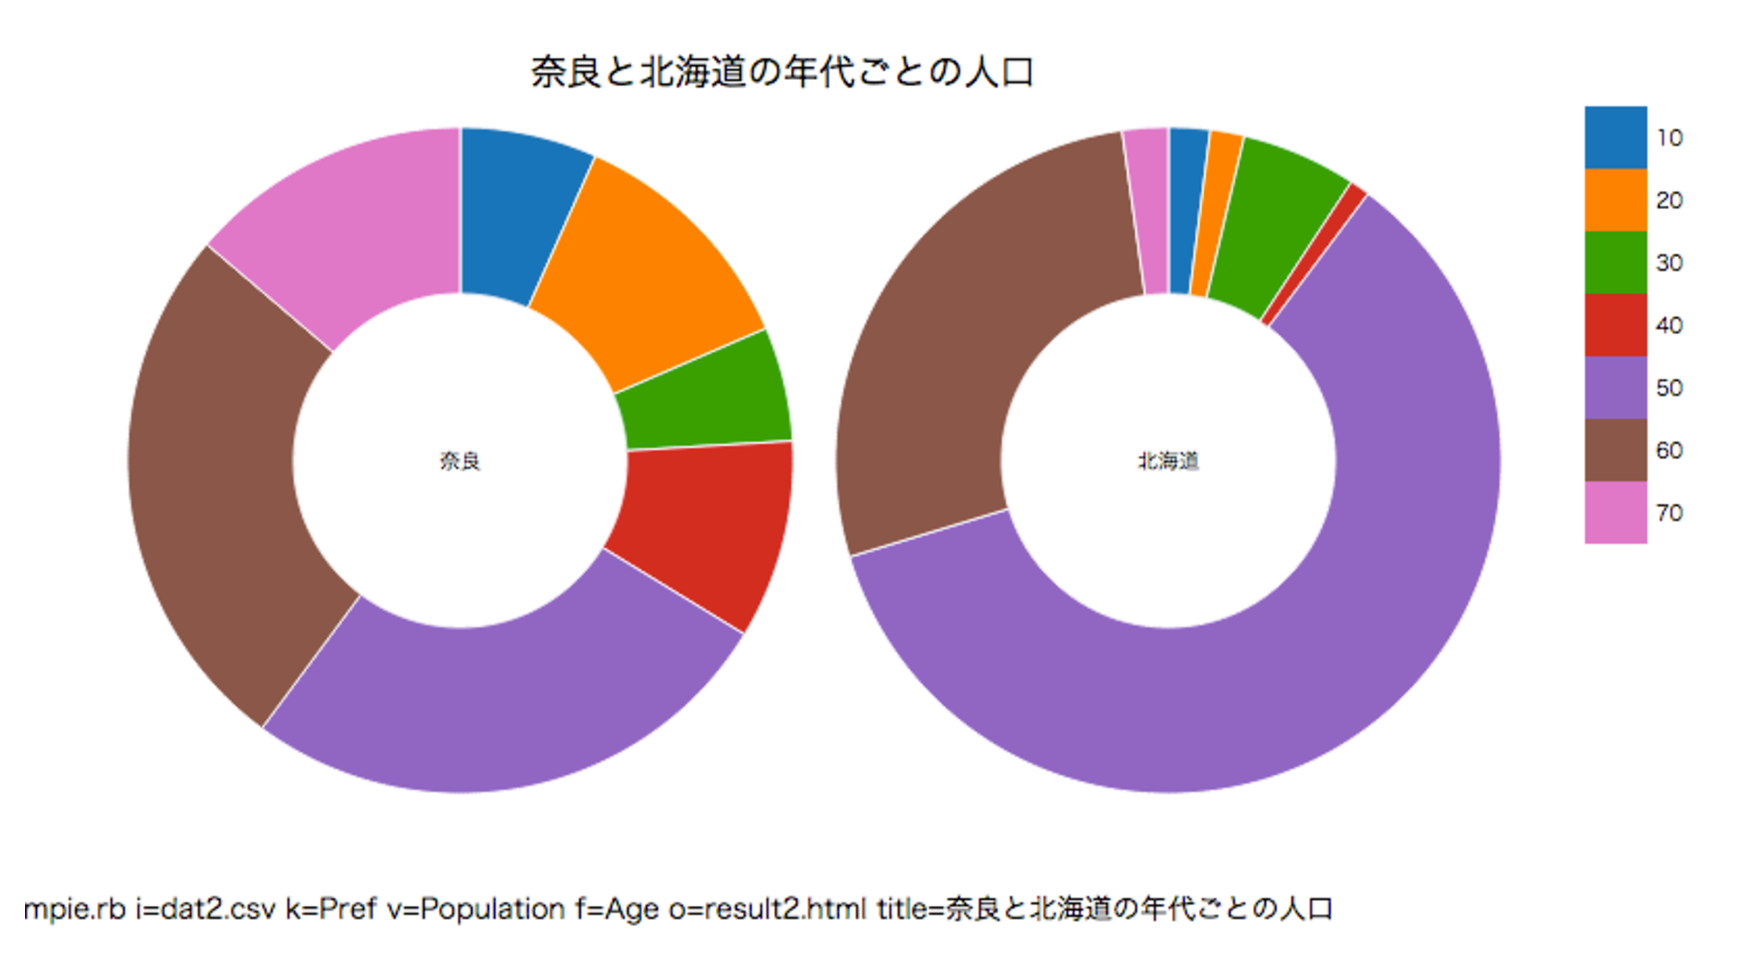
\includegraphics[scale=0.5]{figure/mpie2.eps}
}
\end{flushleft}

\subsubsection*{例3: 2次元の円グラフ行列を描画する}
\verb|dat3.csv|ファイルの\verb|テーマパーク名|を構成要素項目、
\verb|Number|を構成比項目とし、\verb|pr=|パラメータに半径100を指定して円グラフを描画する。
\verb|k=|パラメータに\verb|Gender|と\verb|Age|項目を指定しているので、
\verb|Gender|項目の値をx軸(横方向)に、
\verb|Age|項目の値をy軸(縦方向)に展開した2次元の円グラフ行列が描画される。

\begin{noautoxspacing}
\begin{Verbatim}[baselinestretch=0.5,frame=single]
$ more dat3.csv
Gender,Age,テーマパーク名,Number
男性,30,デズニ,100
男性,30,UFJ,59
男性,30,梅屋敷,180
男性,40,デズニ,200
男性,40,UFJ,3
男性,40,梅屋敷,10
男性,50,デズニ,110
男性,50,UFJ,40
女性,30,梅屋敷,100
女性,30,デズニ,80
女性,30,UFJ,200
女性,40,デズニ,90
女性,40,UFJ,80
女性,40,梅屋敷,120
女性,50,デズニ,99
女性,50,UFJ,80
女性,50,梅屋敷,110
$ mpie.rb i=dat3.csv k=Gender,Age v=Number f=テーマパーク名 o=result3.html
 title=性別と年代ごとのテーマパーク訪問回 pr=100
#END# mpie.rb i=dat3.csv k=Gender,Age v=Number f=テーマパーク名 o=result3.html 
title=性別と年代ごとのテーマパーク訪問回 pr=100;
\end{Verbatim}
\end{noautoxspacing}

以下の円グラフ行列が描画される。

\begin{flushleft}
\fbox{
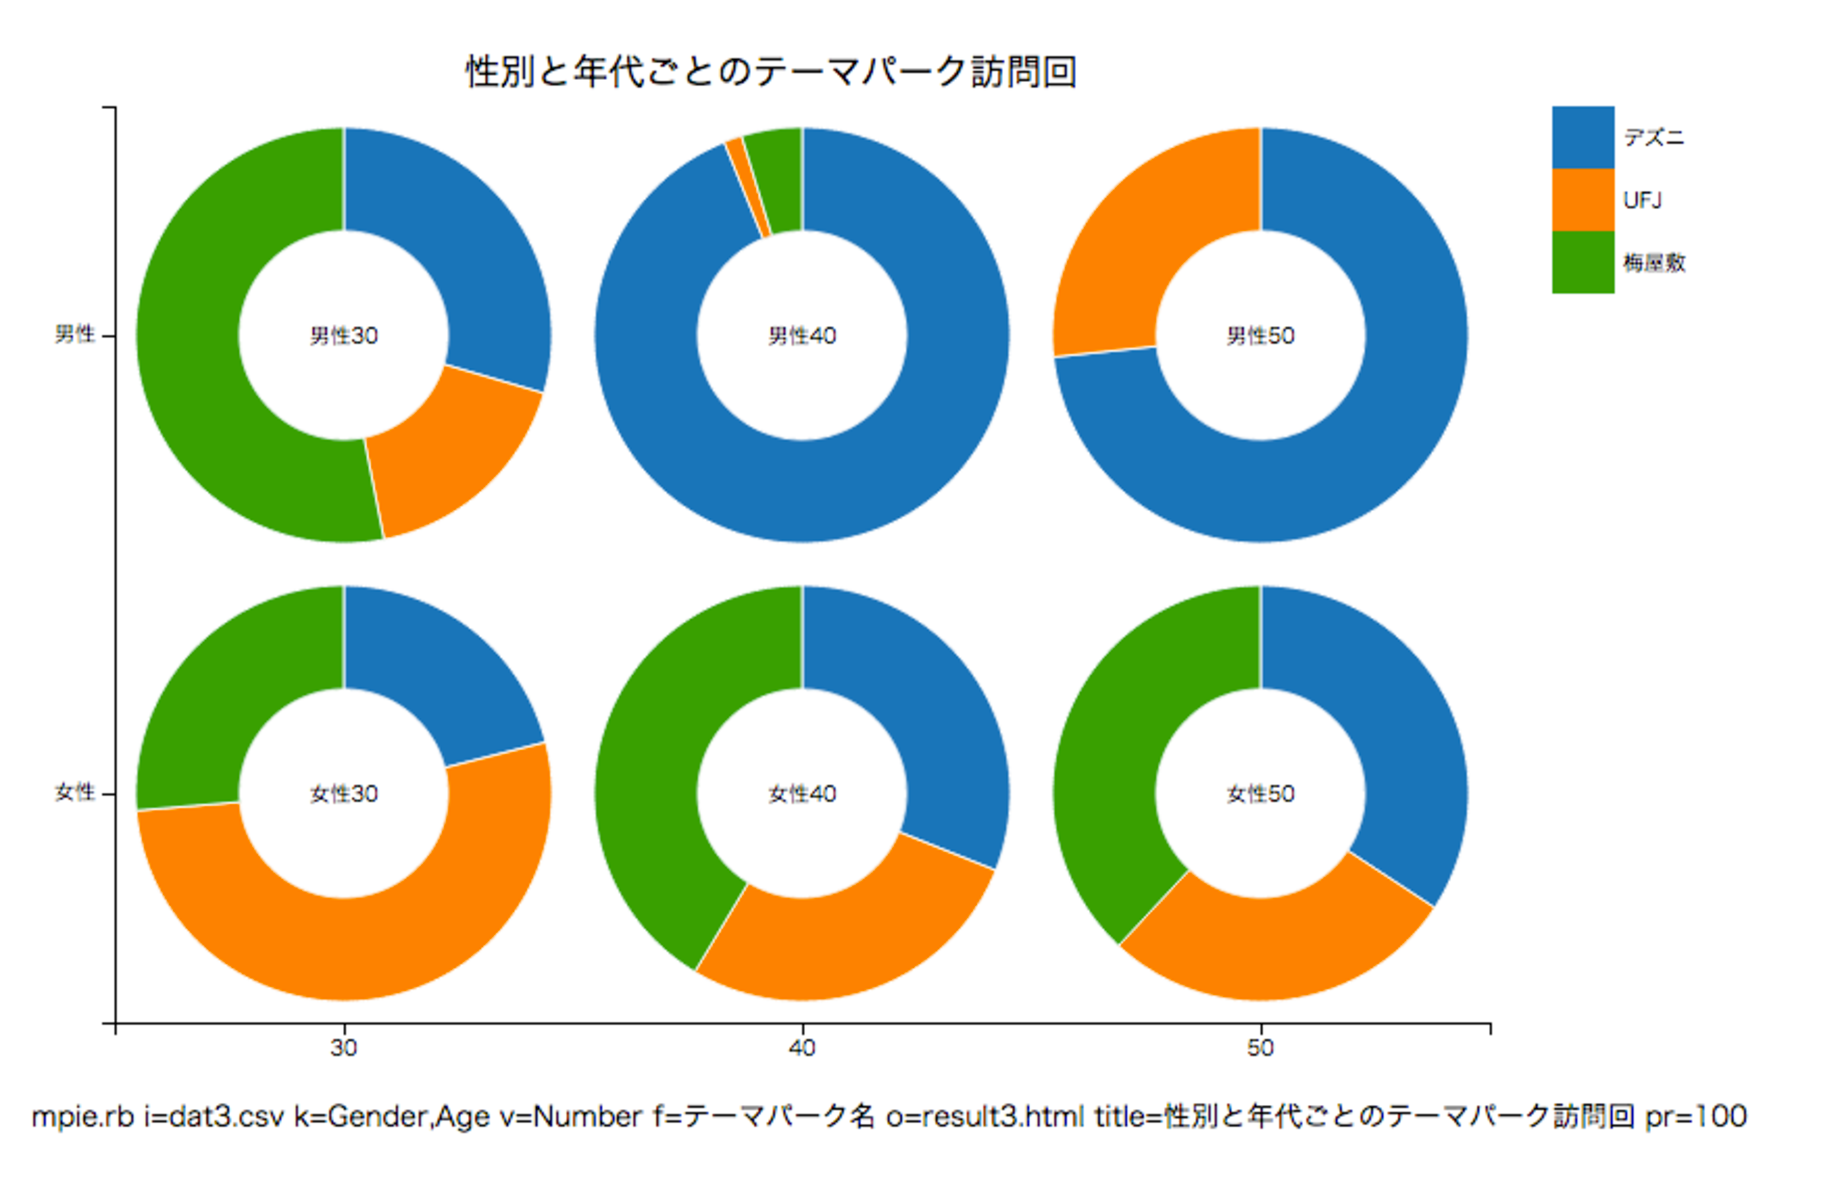
\includegraphics[scale=0.5]{figure/mpie3.eps}
}
\end{flushleft}


%\end{document}

